\chapter{The fundamentals of resilience in cloud computing}
\label{ch:resillience}
Describe resilience now, close some possible routes to take, through writing period


Get a concrete idea what resilience means, underlying concepts


Identify where the strengths of micro services lie compared to monolith.


Set the stage: Why are we talking about resilience, why is it important?



Nygaard describes how software engineering is taught incompletely, and that focus when developing distributed software should be shifted. Nygaard states that focus should be on what a system should not do, contra today's focus on what a system should do. The first acknowledgement when developing distributed systems is according to Nygaard the realisation that failure will occur, and focus should be on handling them instead of avoiding them altogether. Further stating that a stable system will keep on working as intended, even though persistent stress or component failure is present.

\begin{quote_highlight}
"Once you accept that failures will happen, you have the ability to design your system's reaction to specific failures. [..] This sort of self-protection determines the whole system's resilience." \cite[p. 27]{nygard2007release}
\end{quote_highlight}

Strigini describes a movement within information and communication technology, stating that newly developed systems are more interconnected and changed without global system intervention by developers. Setting unprecedented requirements to existing practices of dependable design, making current practices inadequate when trying to deliver satisfactory levels of dependability.

\begin{quote_highlight}
"While existing practices of dependable design deal reasonably well with achieving and predicting dependability in ICT systems that are relatively closed and unchanging, the tendency to making all kinds of ICT systems more interconnected, open, and able to change without new intervention by designers, is making existing techniques inadequate to deliver the same levels of dependability"\cite[p. 5]{strigini2012fault}
\end{quote_highlight}

Dealing with resilience in distributed systems is a necessity, when applications are growing in scale and complexity. The following chapter will establish a definition of resilience, which can be used to evaluate application and infrastructure architecture. 

\subsection{Defining resilience}
Resilience stems from the Latin word resilíre, meaning "to leap back", relating resilience to software engineering it can be defined as a systems ability to "bounce back" and adapt to disruption. \citeauthor{omer2013resilience} Resilience has been used within many disciplines before being applied to software engineering, and has been defined very broadly, incorporating many aspects within a distributed system context. The following section will try to pin down what resilience means in the distributed systems context and what it entails to strive for a  system with a high resilience.


Resilience has been defined and characterised by many different parties, within several disciplines. \cite{folke2002resilience, dalziell2004resilience, rose2005modeling, andersson2006urban, fiksel2003designing, bruneau2003framework, reed2009methodology, pavard2006design}
These definitions help understand the meaning of resilience, and link it to the understanding of cloud computing. Important keywords from the resilience definitions have been identified and put into figure \ref{fig:resilience_keywords}, creating an resilience characteristic overview. The keywords identify core concepts understood when using the word resilience across many disciplines, and are all very relevant when defining resilience within cloud computing. 

All collections of keywords relate very closely, and help define key concepts within resilience with keywords such as: \textit{Stable equilibrium, cope, adapt, proactive measures, reorganize, retain structure, redundancy, robustness}. 

The context in which there is a necessity for resilience is also included and clear, focusing on the possible disruptive events, described with the following keywords: \textit{undergoing change, face of disruption, face of stress, perturbation, disruptive events}, emphasizing the need for resilient systems in environment characterized by these keywords.

\begin{figure}[!htb]
  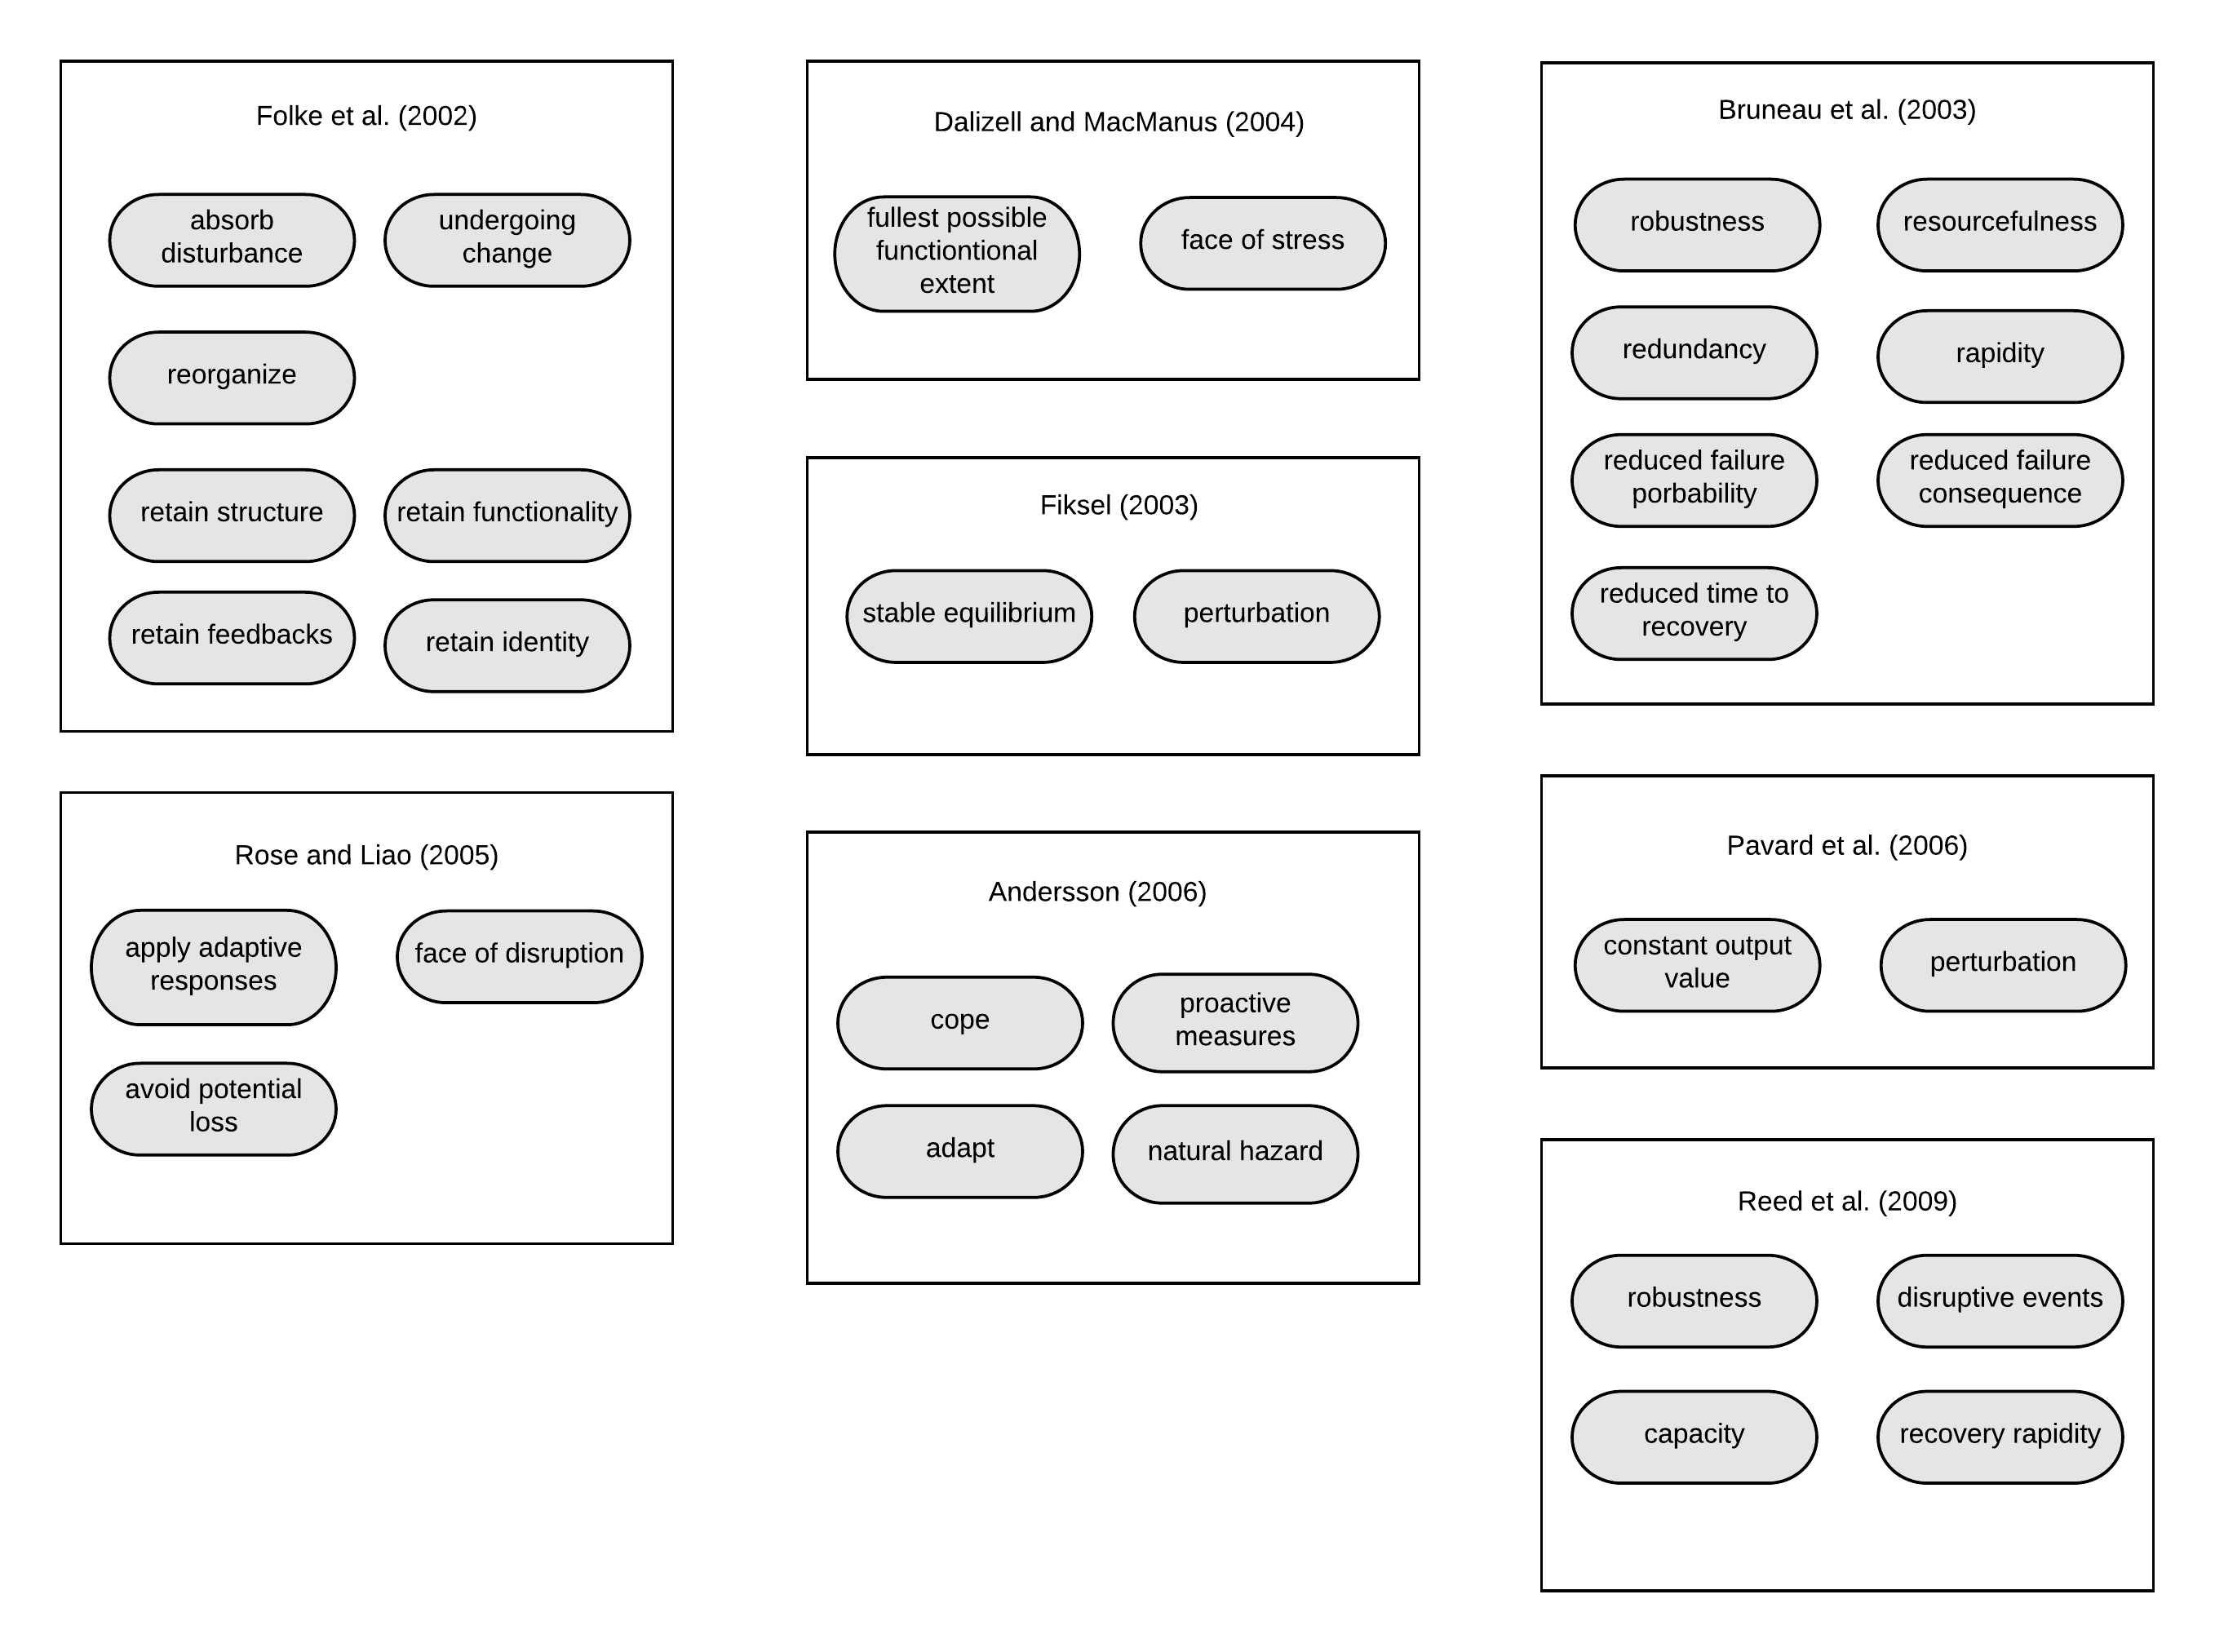
\includegraphics[scale=0.18]{resilience_keywords}  
  \caption{Resilience keywords}
  \label{fig:resilience_keywords}
\end{figure}


The keywords can be grouped and related to know principles within cloud computing, helping simplify the broader characteristics of resilience, creating a model for a cloud computing related resilience definition. The keywords have been grouped according to their association, under a headline inspired directly by the identified resilience keywords and known cloud computing keywords, seen on figure \ref{fig:resilience_keywords_grouped}, the two overarching words being \textit{dependability} and \textit{adaptivity} each with several sub-concepts.




\begin{figure}[!htb]
  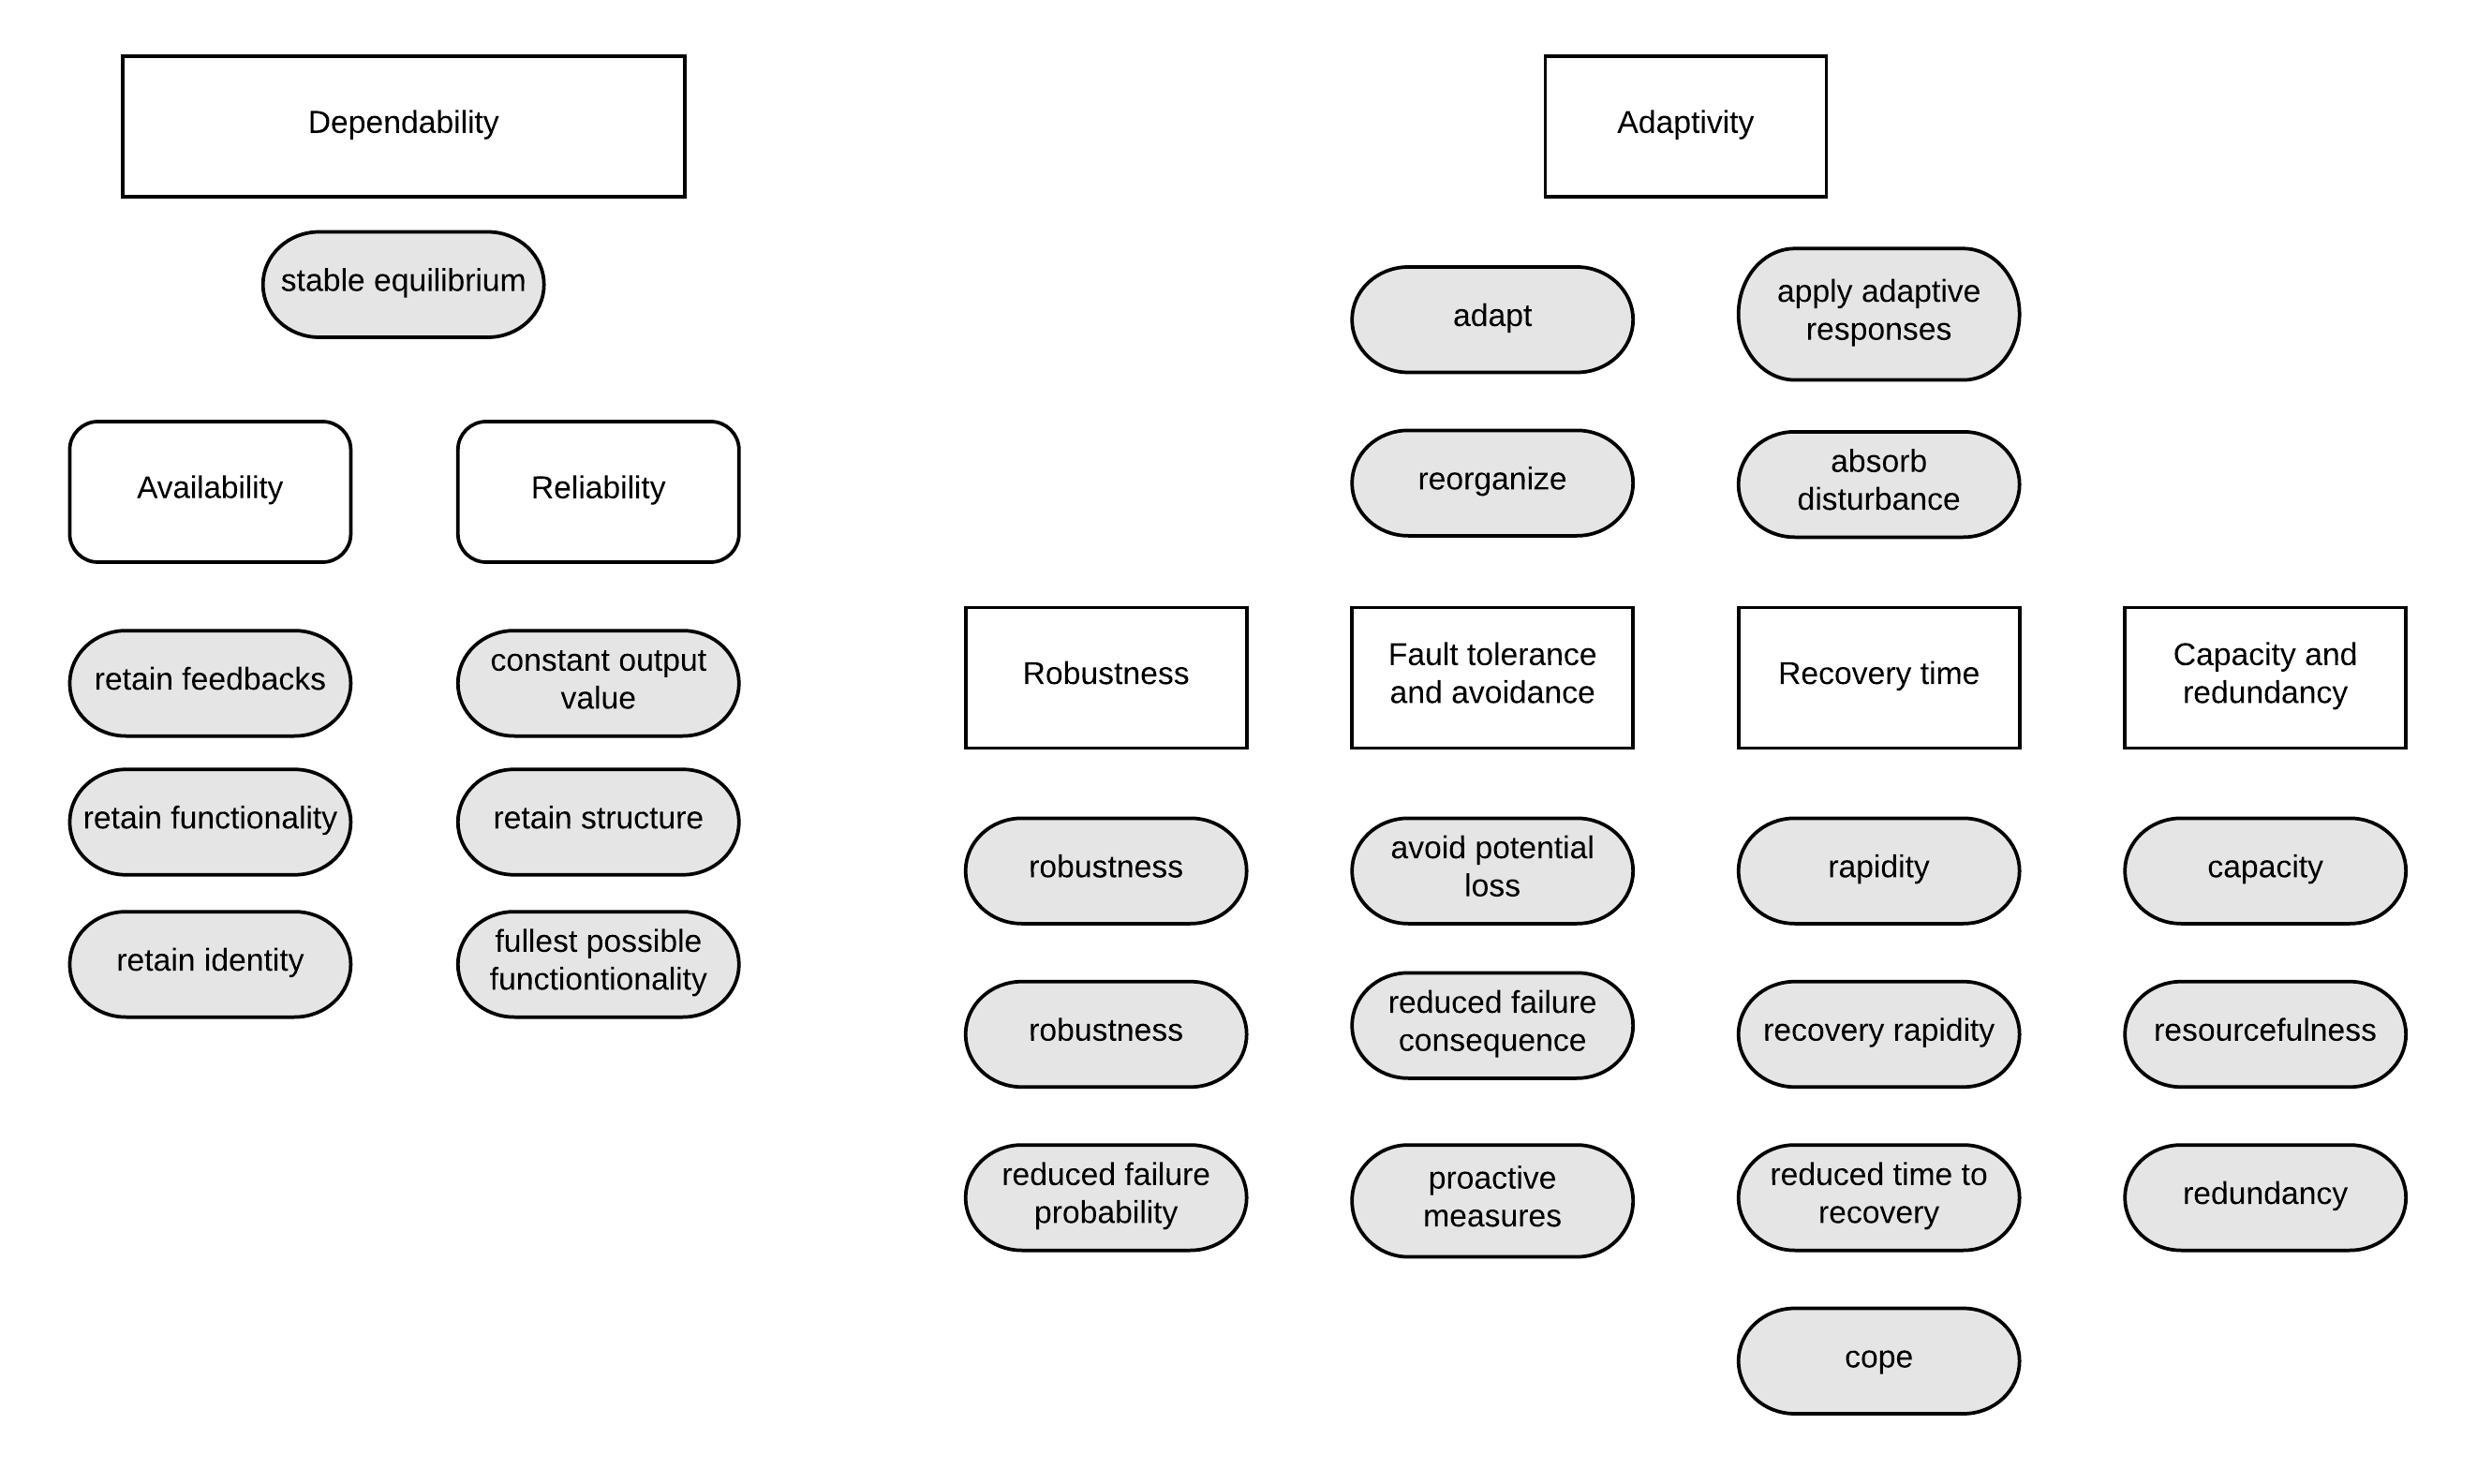
\includegraphics[scale=0.18]{resilience_keywords_grouped}  
  \caption{Resilience keywords grouped in a cloud context}
  \label{fig:resilience_keywords_grouped}
\end{figure}


\comment{Notes}
Resilience is widely used within different disciplines, and can according to \cite[p. 15]{omer2013resilience}, be defined as the following within system engineering.

\begin{quote_highlight}
"Ability of the system to resume normal functionality after shock"\cite[p. 15]{omer2013resilience}
\end{quote_highlight}

\begin{quote_highlight}
"ability to deliver, maintain, improve service when facing threats and evolutionary changes" \cite[p. 4]{strigini2012fault}
\end{quote_highlight}



and can according to \cite[p. 15]{omer2013resilience}, be defined as the following within system engineering. "Ability of the system to resume normal functionality after shock"\cite[p. 15]{omer2013resilience}


\citeauthor{omer2013resilience} 

\cite{omer2013resilience}

"Thus, dependability and resilience in cloud computing are of paramount importance to guarantee availability and reliability of services and application execution, even in the presence of large number of faulty components." \citeauthor{abid2014toward}

\begin{quote_highlight}
"A resilient system keeps processing transactions, even when there are transient impulses, persistent stresses, or component failures disrupting normal processing." \cite[p. 24]{nygard2007release}
\end{quote_highlight}
Resilience can be defined as the capacity to recover quickly, conveys the meaning of "to leap back" "bounce back" after disruption/error


"Here, the word “resilience” is used to identify enhanced ability to deal with the unexpected, or a more flexible approach to achieving safety than the current mainstream approaches"  \cite[p. 5]{strigini2012fault}

"[...] visibly rebounding from deviations and returning to (or continuing in) a desirable way of functioning [...]" \cite[p. 6]{strigini2012fault}





overarching goal of system, continue to function, fullest possible extent, in face of stress, to achieve purpose

proactive preparation and reactive measures, in face of natural hazards


return to stable equilibrium state after disturbance


reduced failure probability, reduced consequences, reduced recovery time


Counterpart to resilience is brittleness, brittle system lack ability to adapt and transmit disruption (onwards in the system i guess)


\cite[p. 4]{omer2013resilience}
"A failure in any one infrastructure could result in cascading failures in other infrastructures. The failure propagate from one element to the next and may have catastrophic consequences. Building resilience into infrastructures prepares the system for mitigating disasters and hence reduces the losses incurred by service disruption"


"The primary factor for implementing resilience in systems is to improve the reaction of the system after the occurrence of disruptions or system shock and improve its ability to resume functionality."

\textbf{Resilience} \cite[p. 5]{newman2015microservices} 
A key concept in resilience engineering is the bulkhead. If one component of a system fails, but that failure doesn’t cascade, you can isolate the problem and the rest of the system can carry on working. Service boundaries become your obvious bulkheads. In a monolithic service, if the service fails, everything stops working. With a monolithic system, we can run on multiple machines to reduce our chance of failure, but with microservices, we can build systems that handle the total failure of services and degrade functionality accordingly.
We do need to be careful, however. To ensure our microservice systems can properly embrace this improved resilience, we need to understand the new sources of failure that distributed systems have to deal with. Networks can and will fail, as will machines. We need to know how to handle this, and what impact (if any) it should have on the end user of our software.
We’ll talk more about better handling resilience, and how to handle failure modes, in Chapter 11.

Knowing how much failure you can tolerate, or how fast your system needs to be, is driven by the users of your system. That in turn will help you understand which techniques will make the most sense for you. That said, your users won’t always be able to articulate what the exact requirements are. So you need to ask questions to help extract the right information, and help them understand the relative costs of providing different levels of service.\cite{newman2015microservices}[p. 206]


\textbf{Cross-functional requirements}\cite{newman2015microservices}[p. 207]
Response time/latency
	How long should various operations take?
	“We expect the website to have a 90th-percentile response time of 2 seconds when handling 200 concurrent connections per second.”


Availability
	Can you expect a service to be down? Is this considered a 24/7 service?


Durability of data
	How much data loss is acceptable? How long should data be kept for? This is highly likely to change on a case-by-case basis. For example, you might choose to keep user session logs for a year or less to save space, but your financial transaction records might need to be kept for many year s.
	
	
Once you have these requirements in place, you’ll want a way to systematically measure them on an ongoing basis. You may decide to make use of performance tests, for example, to ensure your system meets acceptable performance targets, but you’ll want to make sure you are monitoring these stats in production as well!


\textbf{Isolate failure}\cite{newman2015microservices}[p. 248]  - Key, can be used to reason about circuit break
"A microservice architecture can be more resilient than a monolithic system, but only if we understand and plan for failures in part of our system. If we don’t account for the fact that a downstream call can and will fail, our systems might suffer catastrophic cascading failure, and we could find ourselves with a system that is much more fragile than before."


"If we hold the tenets of antifragility in mind, and expect failure will occur anywhere and everywhere, we are on the right track. Make sure your timeouts are set appropriately. Understand when and how to use bulkheads and circuit breakers to limit the fallout of a failing component. Understand what the customer-facing impact will be if only one part of the system is misbehaving. Know what the implications of a network partition might be, and whether sacrificing availability or consistency in a given situation is the right call."

\textbf{Architectural safety measures}\cite{newman2015microservices}[p. 209]
There are a few patterns, which collectively I refer to as architectural safety measures, that we can make use of to ensure that if something does go wrong, it doesn’t cause nasty ripple-out effects. These are points it is essential you understand, and should strongly consider standardizing in your system to ensure that one bad citizen doesn’t bring the whole world crashing down around your ears.


But whatever the cause of the failure, we had created a system that was vulnerable to a cascading failure. A downstream service, over which we had little control, was able to take down our whole system.


\textbf{Defining Stability}\cite{nygard2007release}[p. 24]
"A resilient system keeps processing transactions, even when there are transient impulses, persistent stresses, or component failures disrupting normal processing."

\textbf{Countering Integration Point Problems}\cite{nygard2007release}[p. 44]
"The most effective patterns to combat integration point failures are Circuit Break and Decoupling Middleware"


